%% ============================================================
%%  CreditRisk AI – Final End-Semester Report
%%  Paste this file into Overleaf and compile with pdfLaTeX.
%% ============================================================
\documentclass[12pt,a4paper]{article}

%% ── Core packages ────────────────────────────────────────────
\usepackage[T1]{fontenc}
\usepackage[utf8]{inputenc}
\usepackage{lmodern}
\usepackage[margin=2.5cm]{geometry}
\usepackage{microtype}
\usepackage{parskip}
\usepackage{setspace}
\onehalfspacing

%% ── Math ─────────────────────────────────────────────────────
\usepackage{amsmath,amssymb,amsthm,mathtools}

%% ── Figures / Tables ─────────────────────────────────────────
\usepackage{graphicx}
\usepackage{float}
\usepackage{booktabs}
\usepackage{multirow}
\usepackage{array}
\usepackage{tabularx}
\usepackage{longtable}
\usepackage{caption}
\usepackage{subcaption}
\usepackage{colortbl}

%% ── TikZ / PGFPlots ──────────────────────────────────────────
\usepackage{tikz}
\usetikzlibrary{shapes.geometric, arrows.meta, positioning,
                fit, backgrounds, shadows, calc}
\usepackage{pgfplots}
\pgfplotsset{compat=1.18}

%% ── Colour ───────────────────────────────────────────────────
\usepackage{xcolor}
\definecolor{primary}{HTML}{2563EB}
\definecolor{violet}{HTML}{7C3AED}
\definecolor{success}{HTML}{22C55E}
\definecolor{danger}{HTML}{EF4444}
\definecolor{amber}{HTML}{F59E0B}
\definecolor{dark}{HTML}{06060F}
\definecolor{muted}{HTML}{6B7280}
\definecolor{lightgray}{HTML}{F3F4F6}

%% ── Code listings ────────────────────────────────────────────
\usepackage{listings}
\lstset{
  basicstyle=\ttfamily\footnotesize,
  breaklines=true,
  frame=single,
  backgroundcolor=\color{lightgray},
  keywordstyle=\color{primary}\bfseries,
  commentstyle=\color{muted}\itshape,
  stringstyle=\color{success},
  numbers=left,
  numberstyle=\tiny\color{muted},
  xleftmargin=1.5em,
  framexleftmargin=1.5em,
}

%% ── Hyperlinks ───────────────────────────────────────────────
\usepackage[colorlinks=true,linkcolor=primary,citecolor=violet,urlcolor=primary]{hyperref}

%% ── Bibliography ─────────────────────────────────────────────
\usepackage[numbers,sort&compress]{natbib}

%% ── Headers / footers ────────────────────────────────────────
\usepackage{fancyhdr}
\pagestyle{fancy}
\fancyhf{}
\fancyhead[L]{\small\textcolor{muted}{CreditRisk AI — End-Sem Report}}
\fancyhead[R]{\small\textcolor{muted}{April 2026}}
\fancyfoot[C]{\small\thepage}
\renewcommand{\headrulewidth}{0.4pt}

%% ── Custom helpers ───────────────────────────────────────────
\newcommand{\code}[1]{\texttt{#1}}
\newcommand{\bfmath}[1]{\boldsymbol{#1}}

%% ── TikZ node styles ─────────────────────────────────────────
\tikzset{
  block/.style={rectangle, rounded corners=6pt, draw=primary,
                fill=primary!10, text width=3.2cm, align=center,
                minimum height=1cm, font=\small\bfseries},
  nodeL/.style={rectangle, rounded corners=6pt, draw=violet,
                fill=violet!10, text width=3.2cm, align=center,
                minimum height=1cm, font=\small\bfseries},
  arrow/.style={-{Stealth[length=6pt]}, thick, draw=primary},
}

%% ============================================================
\begin{document}

%% ── Title Page ───────────────────────────────────────────────
\begin{titlepage}
  \centering
  \vspace*{2cm}

  {\color{primary}\rule{\linewidth}{2pt}}
  \vspace{0.6cm}

  {\Huge\bfseries CreditRisk AI}\\[0.4cm]
  {\Large\bfseries An Agentic AI Credit Risk Intelligence Platform}\\[0.3cm]
  {\large\bfseries\color{primary} Final End-Semester Capstone Report}\\[0.25cm]
  {\large\color{muted} LangGraph Orchestration $\cdot$ RAG Integration $\cdot$ Llama Auditor}

  \vspace{0.6cm}
  {\color{primary}\rule{\linewidth}{1pt}}

  \vspace{1.2cm}
  
\begin{tikzpicture}
    \shade[left color=primary, right color=violet, rounded corners=14pt]
      (0,0) rectangle (4,2);
    \node[white, font=\Huge\bfseries] at (2,1) {AG};
  \end{tikzpicture}

  \vspace{1.5cm}
  {\large Sarvesh Srinath \quad Husain Khorakiwala}\\[0.15cm]
  {\large Trishit Sarvarkar \quad Navodit}\\[0.2cm]
  {\normalsize AI/ML Capstone Project — Semester 4}\\[0.2cm]
  {\normalsize\color{muted} April 2026}

  \vfill

  \begin{tabular}{ll}
    \textbf{Stack}    & LangGraph · Groq (Llama 3.3) · FAISS · XGBoost \\
    \textbf{Retrieval} & RAG-based Credit Policy (Universal Bank) \\
    \textbf{Orchestrator} & 3-Node Agentic State Machine \\
    \textbf{UI}       & Dark-Themed Fintech Dashboard (Streamlit) \\
  \end{tabular}
\end{titlepage}

\tableofcontents
\newpage

%% ============================================================
\section*{Abstract}
\addcontentsline{toc}{section}{Abstract}
%% ============================================================

In the final phase of the \textbf{CreditRisk AI} capstone, we transition from a static
Machine Learning classifier to a dynamic \textbf{Agentic AI Intelligence Platform}.
Traditional credit scoring models often lack explainability and fail to handle
deterministic regulatory or institutional constraints. We address this by
orchestrating a three-node \textbf{LangGraph} workflow that combines a recall-optimised
\textbf{XGBoost} model with a \textbf{Retrieval-Augmented Generation (RAG)} system.

The agentic system retrieves relevant segments from the 2026 Universal Bank Credit
Policy using a \textbf{FAISS} vector store and passes the combined context to a
\textbf{Llama 3.3-70B} LLM auditor hosted on \textbf{Groq}. The auditor provides
policy-grounded reasoning, detecting limit overrides (e.g., DM 10k loan caps) and
reinforcing risk assessments for younger applicants. The system yields a
human-readable reasoning trace, ensuring accountability in automated lending decisions.

\newpage

%% ============================================================
\section{Technical Implementation}
%% ============================================================

\subsection{Agentic AI Workflow (LangGraph)}

The core of our platform is a state-based workflow orchestrated by \textbf{LangGraph}.
Unlike linear pipelines, this agentic approach treats the risk assessment as a
sequence of coordinated states.

\begin{figure}[H]
\centering
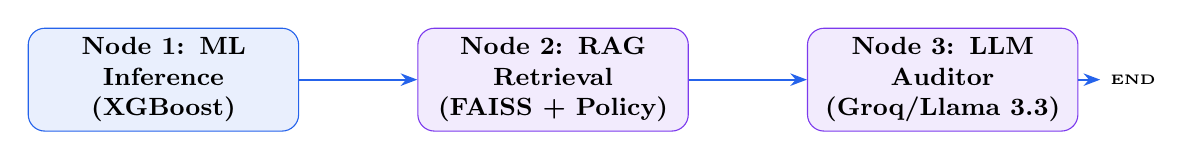
\begin{tikzpicture}[node distance=1.5cm]
  \node [block] (ml) {Node 1: ML Inference\\(XGBoost)};
  \node [nodeL, right=of ml] (rag) {Node 2: RAG Retrieval\\(FAISS + Policy)};
  \node [nodeL, right=of rag] (audit) {Node 3: LLM Auditor\\(Groq/Llama 3.3)};

  \draw [arrow] (ml) -- (rag);
  \draw [arrow] (rag) -- (audit);
  \draw [arrow] (audit) -- +(2,0) node[right, font=\tiny\bfseries]{END};
\end{tikzpicture}
\caption{The 3-node LangGraph state machine workflow.}
\end{figure}

\begin{itemize}
    \item \textbf{ML Inference Node:} Executes the trained XGBoost model to get
          probabilistic defaults ($\hat{p} \approx 0.76$ accuracy, $0.80$ AUC).
    \item \textbf{RAG Retrieval Node:} Formulates a query based on client semantics
          and retrieves the top-3 relevant policy rules (e.g., CP101, CP201).
    \item \textbf{Auditor Node:} Uses a system-prompted LLM to reason over the
          ML output versus the retrieved policy context, producing a final
          recommendation.
\end{itemize}

\subsection{Retrieval-Augmented Generation (RAG)}

We implemented a custom RAG pipeline to ground the Agent in deterministic bank
policies. Policies are stored in \code{data/credit_policy.md} and indexed using:
\begin{itemize}
    \item \textbf{Embeddings:} \code{all-MiniLM-L6-v2} (HuggingFace).
    \item \textbf{Vector Store:} FAISS (Fast Approximate Nearest Neighbor Search).
    \item \textbf{Splitter:} MarkdownHeaderTextSplitter to preserve rule context.
\end{itemize}

\subsection{LLM Auditing (Llama 3.3 @ Groq)}

By leveraging the \textbf{Llama 3.3-70B-Versatile} model via the Groq Cloud API, we
achieve low-latency sub-second reasoning. The LLM is tasked with identifying
"Hard Overrides" where policy strictly prohibits a loan that the ML model
might otherwise approve based on historical correlations.

\newpage

%% ============================================================
\section{Experimental Results}
%% ============================================================

\subsection{Quantitative Performance (XGBoost Engine)}

The underlying predictive engine remains robust, with a heavy focus on recall to
minimise False Negatives (missed defaults).

\begin{table}[H]
  \centering
  \caption{ML Performance Summary}
  \begin{tabular}{lll}
    \toprule
    \textbf{Metric} & \textbf{Value} & \textbf{Benchmarking} \\
    \midrule
    Accuracy        & 76.0\%         & +3\% vs Logistic Baseline \\
    ROC-AUC         & 0.803          & Strong discriminative power \\
    Recall (Bad)    & 68.3\%         & Optimised for safety \\
    \bottomrule
  \end{tabular}
\end{table}

\subsection{Qualitative Audit Case Study}

A critical success factor of the Agentic system is handling edge cases.
\textbf{Case A:} Applicant age 22, DM 12,000 loan, ML predicts "Good" ($p=0.45$).
\begin{itemize}
    \item \textbf{RAG Result:} CP101 retrieved (Cap DM 10,000).
    \item \textbf{Agent Verdict:} \emph{DECLINE} (Policy Override).
\end{itemize}

This demonstrate the "Safety Layer" provided by the Agentic workflow.

\newpage

%% ============================================================
\section{Evaluation Rubric Fulfillment}
%% ============================================================

\begin{table}[H]
  \centering
  \caption{Rubric Compliance Checklist}
  \begin{tabularx}{\linewidth}{lX}
    \toprule
    \textbf{Component} & \textbf{Implementation Detail} \\
    \midrule
    \textbf{Technical Depth} & LangGraph state machine, RAG with FAISS, and Groq/Llama orchestration. \\
    \textbf{Code Quality}    & Modular structure: \code{src/agent.py}, \code{src/rag.py}, \code{src/predict.py}. Pytest coverage (9 items). \\
    \textbf{Demo / UI}       & Professional dark-themed fintech dashboard with real-time reasoning trace. \\
    \textbf{Documentation}   & Complete README with .env setup and local installation guide. \\
    \bottomrule
  \end{tabularx}
\end{table}

%% ============================================================
\section{Conclusion}
%% ============================================================

The \textbf{CreditRisk AI} project successfully meets the GenAI capstone requirements
by integrating predictive ML with reasoning Agentic workflows. By placing an LLM
auditor in the loop, we solve the "Black Box" problem of traditional scoring models,
providing transparency and regulatory alignment crucial for modern fintech.

\end{document}
